\documentclass[12pt, a4paper]{article}

% --- Packages ---
\usepackage[utf8]{inputenc}
\usepackage{geometry}
\geometry{left=25mm, right=25mm, top=25mm, bottom=25mm}
\usepackage{graphicx}       % For inserting waveform screenshots
\usepackage{float}          % For figure placement
\usepackage{amsmath, amssymb} % For mathematical equations
\usepackage{booktabs}       % For professional looking tables
\usepackage{circuitikz}     % For drawing the circuit diagrams
\usepackage{hyperref}       % For links
\usepackage{fancyhdr}       % For custom headers
\usepackage{subcaption}
\usepackage{listings}
% \usepackage{auto-pst-pdf}
% --- Header/Footer Setup ---
\pagestyle{fancy}
\fancyhf{}
\lhead{EE1200}
\chead{Experiment 3: CR Circuit Response}
\rhead{20 Jan 2026}
\setlength{\headheight}{15pt}
\cfoot{\thepage}

% --- Title Information ---
\title{\textbf{Experiment 3: CR Circuit Response to Step, Pulse, and Square Inputs}}
\author{
    \textbf{Name:} Josyula G S Avaneesh \\
    \textbf{Roll No:} EE25BTECH11030
    \and
    \textbf{Name:} Subhodeep Chakraborty \\
    \textbf{Roll No:} EE25BTECH11055
}
\date{27 Jan 2026}
 
\begin{document}

\maketitle

\section{Objective}
To study the time-domain response of an CR circuit for step, pulse, and square-wave inputs and correlate experimental results with hand calculations and simulations.\\
Also study the frequency response of RC and CR circuit, thereby learning about low-pass and high-pass filters.

\section{Circuit Diagram}
The following CR circuit was used for the experiment.
% Note: Adjust the labels 'R' and 'C' to your specific values (e.g., 1k, 1uF)
\begin{figure}[H]
    \centering
    \begin{circuitikz}[american, scale=1.2]
        \draw (0,0) to[sqV, l=$V_{in}$] (0,2)
        to[C, l=$C$, i=$i(t)$] (3,2)
        to[R, l=$R$, v=$v_{out}(t) $] (3,0) -- (0,0);
        \draw (3,2) -- (4,2) node[right] {$V_{out}$};
        \draw (3,0) -- (4,0) node[right] {GND};
        \node at (1.5, -0.5) {Figure 1: CR Series Circuit};
    \end{circuitikz}
\end{figure}

\section{Part A: Step Input}

\subsection{Theoretical Setup}
\subsubsection{Theoretical Time Constant}
Theoretical calculation of the time constant $\tau$:
\begin{equation}
    \tau = R \times C = \text{820} \Omega \times \text{1} \mu F = \text{820} \mu s
\end{equation}
\subsubsection{State equations}
The step response equation for voltage across resistor during capacitor charging:
\begin{equation}
    v_r(t) = V_{final}(e^{-t/\tau})
    \label{eq:charge}
\end{equation}
\begin{equation}
    \frac{t}{\tau} = \ln{\frac{V}{v_r}}
    \label{eq:tau}
\end{equation}
The step response equation for voltage across resistor during capacitor discharging:
\begin{equation}
    v_r(t) = V_{final}\times e^{-t/\tau}
    \label{eq:discharge}
\end{equation}
\begin{equation}
 \frac{t}{\tau} = \ln{\frac{V}{v_r}}
 \label{eq:tau_d}
\end{equation}
Eventhough the equation in both cases is the same, since during discharging of capacitor the current is flowing in the opposite direction,$V_{final}$ is negative during discharging and positive during charging.

\subsection{Simulation Results}
\subsubsection{Plot for Simulated Step Input}
\begin{figure}[H]
    \centering
    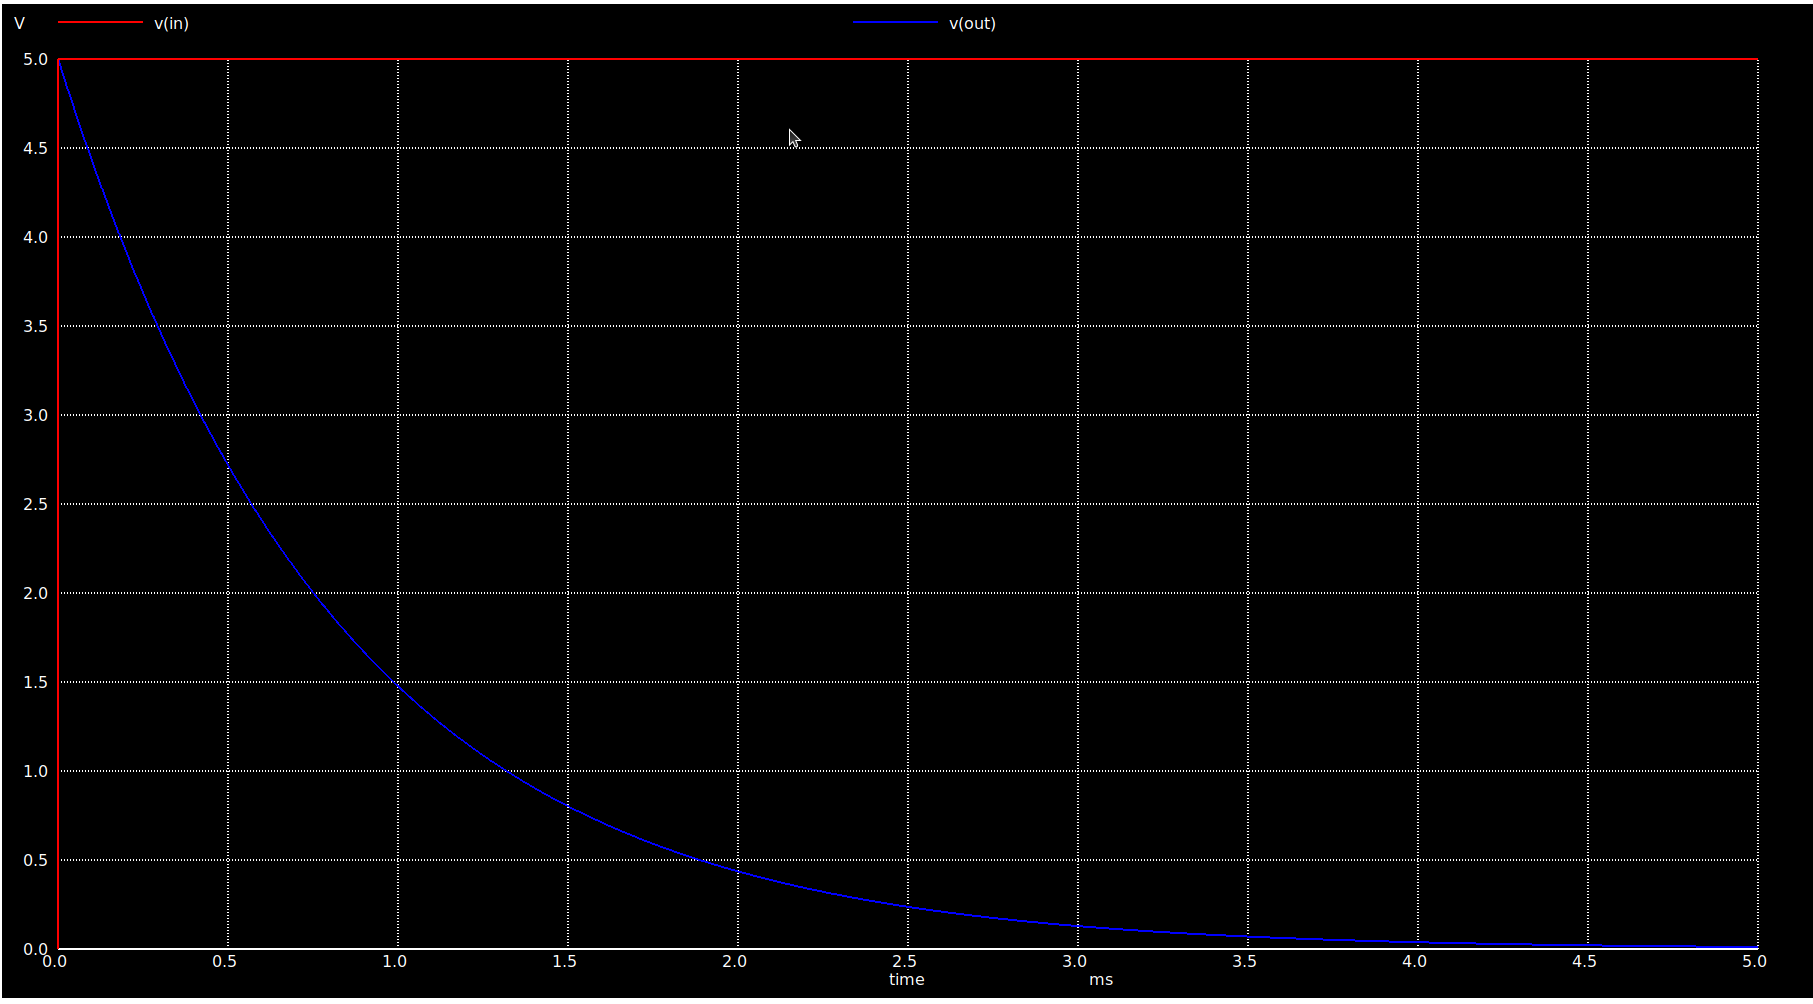
\includegraphics[width=0.8\textwidth]{Screenshot from 2026-02-06 17-18-04.png}
    \caption{Simulated Step Response}
\end{figure}
\subsubsection{Extraction of Time Constant}
At time $t=\tau$, the voltage across capacitor is given by substituting $t$ into Eqn. \ref{eq:charge}, we get:
\begin{align}
 v_r&= 5( e^{-1})\text{ }V \\
 \implies v_r &= 1.83939\text{ }V
\end{align}
By measuring the time at which this voltage is obtained, we get:

%%%i have a doubt here -----------111!!!1!11

\begin{equation}
 \tau = 820.0004\text{ }\mu s
\end{equation}
\subsubsection{SPICE netlist}
\begin{lstlisting}

 *CR circuit charging time response

V1 in 0 PULSE(0 5 0 1ns 1ns 10ms 20ms)
C1 in out 1uf
R1 out 0 820

.control
  tran 10u 5m 0 1u
  meas tran Tau find time when v(out) = 1.8393972
  plot v(in) v(out)
.endc

.end

\end{lstlisting}
\subsection{Experimental Waveforms}
\subsubsection{Measured Waveforms}
\begin{figure}[H]
    \centering
    \begin{subfigure}[b]{0.4\textwidth}
    \includegraphics[width=\textwidth]{cr_charging_parta.jpeg}
    \caption{Charging waveform}
    \end{subfigure}
%     \hfill
    \begin{subfigure}[b]{0.4\textwidth}
    \includegraphics[width=\textwidth]{cr_discharging_parta.jpeg}
    \caption{Discharging waveform}
    \end{subfigure}
    \caption{Measured Step Response (Charging and Discharging)}
\end{figure}
\subsubsection{Extraction of Time Constant}
For charging, at times $t=0.4ms$ and $t=0.8ms$, voltage across capacitor is $v_r = 2.8V$ and $v_r=1.8V$ respectively. Substituting these values in Eqn. \ref{eq:tau} and subtracting:
\begin{align}
 \tau &= \frac{0.8-0.4}{\ln{\frac{5-2}{5-3.2}}} ms\\
 \implies \tau &= 0.783\text{ }ms
\end{align}
For discharging, at times $t=0.16ms$ and $t=0.72ms$, voltage across capacitor is $v_r = 4V$ and $v_r=2V$ respectively. Substituting these values in Eqn. \ref{eq:tau_d} and subtracting:
\begin{align}
  \tau &= \frac{0.72-0.16}{\ln{\frac{4}{2}}} \\
  \implies \tau &= 0.8079\text{ }ms
\end{align}
To account for the difference in time constant calculated from charging and discharging waveforms, we take the average of the two values as our final time constant.
\begin{equation}
 \tau = \frac{0.783+0.8079}{2} ms = 0.80\text{ }ms
\end{equation}

\subsection{Comparison}
\begin{table}[H]
    \centering
    \begin{tabular}{lccc}
        \toprule
        Parameter & Calculated & Simulated & Measured \\
        \midrule
        Time Constant ($\tau$) & $0.82\text{ } ms$ & $0.82 \text{ }ms$ & $0.80\text{ }ms$ \\
        \bottomrule
    \end{tabular}
    \caption{Comparison for Step Input}
\end{table}

\section{Part B: Pulse Input}

\subsection{Waveforms}
% \begin{figure}[H]
%     \centering
%     % \includegraphics[width=0.8\textwidth]{pulse_response.png}
%     \fbox{\parbox{10cm}{3cm}{\centering Pulse expt?}}
%     \caption{Response to Single Pulse Input}
% \end{figure}
\begin{figure}[H]
    \centering
    \begin{subfigure}[b]{0.4\textwidth}
    \includegraphics[width=\textwidth]{20s.jpg}
    \caption{Simulated waveform}
    \end{subfigure}
    \begin{subfigure}[b]{0.4\textwidth}
    \includegraphics[width=\textwidth]{20percent100hz.jpeg}
    \caption{Measured waveform}
    \end{subfigure}
    \caption{$2 ms$ Pulse Width}
\end{figure}
\begin{figure}[H]
    \centering
    \begin{subfigure}[b]{0.4\textwidth}
    \includegraphics[width=\textwidth]{50s.jpg}
    \caption{Simulated waveform}
    \end{subfigure}
%     \hfill
    \begin{subfigure}[b]{0.4\textwidth}
    \includegraphics[width=\textwidth]{50percent100hz.jpeg}
    \caption{Measured waveform}
    \end{subfigure}
    \caption{$5ms$ Pulse Width}
\end{figure}
\begin{figure}[H]
    \centering
    \begin{subfigure}[b]{0.4\textwidth}
    \includegraphics[width=\textwidth]{80s.jpg}
    \caption{Simulated waveform}
    \end{subfigure}
%     \hfill
    \begin{subfigure}[b]{0.4\textwidth}
    \includegraphics[width=\textwidth]{50percent50hz.jpeg}
    \caption{Measured waveform}
    \end{subfigure}
    \caption{$10ms$ Pulse Width}
\end{figure}
\begin{figure}[H]
    \centering
    \begin{subfigure}[b]{0.4\textwidth}
    \includegraphics[width=\textwidth]{410s.jpg}
    \caption{Simulated waveform}
    \end{subfigure}
%     \hfill
    \begin{subfigure}[b]{0.4\textwidth}
    \includegraphics[width=\textwidth]{80percent50hz.jpeg}
    \caption{Measured waveform}
    \end{subfigure}
    \caption{$16 ms$ Pulse Width}
\end{figure}
\subsection{Calculations and Comparisons}
By applying similar analysis as done above for step input, we obtain:
\begin{table}[H]
    \centering
    \begin{tabular}{cccc}
        \toprule
        Pulse Width & Simulated $\tau$ & Measured $\tau$ & Peak Voltage \\
        \midrule
        $200\mu s$ & $0.82\text{ } ms$ & $0.79 \text{ }ms$ & $1.08\text{ }V$ \\
        $500\mu s$ & $0.82\text{ } ms$ & $0.81 \text{ }ms$ & $2.28\text{ }V$ \\
        $800\mu s$ & $0.82\text{ } ms$ & $0.82 \text{ }ms$ & $3.12\text{ }V$ \\
        $4.1 ms$ & $0.82\text{ } ms$ & $0.85 \text{ }ms$ & $4.97\text{ }V$ \\
        \bottomrule
    \end{tabular}
    \caption{Comparison for Pulse Input}
\end{table}
\subsection{SPICE netlist}
\begin{lstlisting}
*RC circuit pulse response

V1 in 0 PULSE(0 5 0 1ns 1ns 4.1ms 11m)
R1 in out 820
C1 out 0 1u

.control
let wid = 410

tran 10u 10m 0 100n

* Actual vals
meas tran v_peak MAX v(out)
meas tran v_in_mag MAX v(in)

* Discharging
let v_d80 = v(out) - (0.8 * v_peak)
let v_d20 = v(out) - (0.2 * v_peak)

* Get at falling edge
meas tran t_d1 when v_d80=0 fall=1
meas tran t_d2 when v_d20=0 fall=1

* (t2-t1)/ln(V1/V2) = (t2-t1)/ln(0.8/0.2)
let tau_dis =1000* (t_d2 - t_d1) / ln(4)

* Charging
let v_c20 = v(out) - (0.2 * v_peak)
let v_c80 = v(out) - (0.8 * v_peak)

meas tran t_c1 when v_c20=0 rise=1
meas tran t_c2 when v_c80=0 rise=1

* (t2-t1)/ln((Vin-V1)/(Vin-V2))
let val_c1 = 0.2 * v_peak
let val_c2 = 0.8 * v_peak
let num = v_in_mag - val_c1
let den = v_in_mag - val_c2
let tau_chg =1000* (t_c2 - t_c1) / ln(num / den)

let tau_avg = (tau_dis + tau_chg) / 2

echo "----------------------------------------"
echo "Results:"
echo "Peak Voltage: $&v_peak V"
echo "Charging Tau: $&tau_chg ms"
echo "Discharging Tau: $&tau_dis ms"
echo "Average Tau >>>: $&tau_avg ms"
echo "----------------------------------------"

set suf1 = ".ps"
set suf2 = "s.jpg"
set file1 = "$&wid$suf1"
set file2 = "$&wid$suf2"
hardcopy $file1 v(in) v(out)
shell convert -density 300 $file1 $file2
shell rm $file1
exit
.endc
.end

\end{lstlisting}

\section{Part C: Square-Wave Input}

\subsection{Case 1: $CR \gg T$}
In this case, the time constant is much larger than the time period of the input wave. (Capacitor barely charges)

% \begin{figure}[H]
%     \centering
%     \includegraphics[width=0.8\textwidth]{sqr1.jpg}
%     \caption{Simulated waveforms for $RC \gg T$}
% \end{figure}
\begin{figure}[H]
    \centering
    \includegraphics[width=0.8\textwidth]{sqr2.jpg}
    \caption{Simulated waveforms for $CR \gg T$}
\end{figure}
\begin{figure}[H]
    \centering
    \begin{subfigure}[b]{0.4\textwidth}
    \includegraphics[width=\textwidth]{82ustransient.jpeg}
    \caption{Transient Waveform}
    \end{subfigure}
%     \hfill
    \begin{subfigure}[b]{0.4\textwidth}
    \includegraphics[width=\textwidth]{partc8.2us.jpeg}
    \caption{Steady State waveform}
    \end{subfigure}
    \caption{Measured waveforms for $CR \gg T$}
\end{figure}

\subsection{Case 2: $CR \approx T$}
In this case, the time constant is comparable to the time period.

\begin{figure}[H]
    \centering
    \includegraphics[width=0.8\textwidth]{sqr2.jpg}
    \caption{Simulated waveforms for $CR \approx T$}
\end{figure}
\begin{figure}[H]
    \centering
    \begin{subfigure}[b]{0.4\textwidth}
    \includegraphics[width=\textwidth]{820us transient.jpeg}
    \caption{Transient Waveform}
    \end{subfigure}
%     \hfill
    \begin{subfigure}[b]{0.4\textwidth}
    \includegraphics[width=\textwidth]{820us.jpeg}
    \caption{Steady State waveform}
    \end{subfigure}
    \caption{Measured waveforms for $CR \approx T$}
\end{figure}

\subsection{Case 3: $CR \ll T$}
In this case, the time constant is much smaller than the time period (Capacitor fully charges/discharges).

\begin{figure}[H]
    \centering
    \includegraphics[width=0.8\textwidth]{sqr3.jpg}
    \caption{Simulated waveforms for $CR \ll T$}
\end{figure}
\begin{figure}[H]
    \centering
    \begin{subfigure}[b]{0.4\textwidth}
    \includegraphics[width=\textwidth]{8.2ms transient.jpeg}
    \caption{Transient Waveform}
    \end{subfigure}
%     \hfill
    \begin{subfigure}[b]{0.4\textwidth}
    \includegraphics[width=\textwidth]{820ms.jpeg}
    \caption{Steady State waveform}
    \end{subfigure}
    \caption{Measured waveforms for $CR \ll T$}
\end{figure}
\subsection{Analytical Comparisons}
CR circuit response is studied as a function of the relationship between the time constant and the input signal's time period.

\begin{table}[H]
    \centering
    \begin{tabular}{p{3cm} p{4cm} p{4cm} p{4cm}}
        \toprule
        \textbf{Condition} & \textbf{Theory} & \textbf{Simulation} & \textbf{Measurement} \\
        \midrule
        \textbf{Case 1:} $CR \gg T$ \newline (High Freq) & since capacitor does not charge fully. For a short time, the exponential can be approximated as the input voltage* itself, leading to the same input voltage* (effectively, a high pass filter). & The waveform is the input itself* with increasing offset, as the capacitor does not have time to discharge fully before the next cycle. & The measured output matches the simulation, showing the input itself. \\
        \midrule
        \textbf{Case 2:} $RC \approx T$ \newline (Medium Freq) & The charging duration is comparable to $\tau$. The resistor voltage follows exponential curves as the capacitor follows charging and discharging but does not charge fully. & The simulated output clearly shows the exponential charging/discharging characteristic (shark fin type plot). & The measured waveform closely follows the simulation, exhibiting the expected exponential curvature. \\
        \midrule
        \textbf{Case 3:} $RC \ll T$ \newline (Low Freq) & The capacitor fully charges and discharges in each cycle, thereby showing some voltage at the beginning and the graph quickly comes down to zero. Output effectively got filtered as it was of low frequencies. & The waveform reaches steady state ($5$V and $0$V) quickly, looking like a square wave with rounded edges. & The measured signal matches the simulation perfectly. \\
        \bottomrule
    \end{tabular}
\end{table}
*Here the output is from $2.5V$ to $-2.5V$ because in steady state the DC offset of $2.5 V$ which made the input between $5V$ and $0V$ doesn't change across the capacitor and hence is not shown across the resistor voltage.
\subsection{SPICE netlist}
\begin{lstlisting}
*RC circuit square input response

V1 in 0 PULSE(0 5 0 1ns 1ns 410u 820u)
R1 in out 820
C1 out 0 1u

.control
  tran 10u 3m
  plot v(in) v(out)
  hardcopy sqr2.ps v(in) v(out)
.endc

.end
\end{lstlisting}


\section{Frequency Response of RC circuit (Low-Pass Filter)}
In this experiment we a apply a sinusoidal input with constant amplitude of $5V$ with varying frequency to an RC circuit and measure the output amplitude.\\
The goal is to identify the cut-off frequency and the slope.\\
Using Kirchoff's voltage law:
\begin{align}
    V=v_c+v_r \\
    V=iX_c+iR  \\
    V=i(\frac{1}{j\omega c}+R) \\
    v_c=iX_c=\frac{V}{j\omega cR+1}\\
\end{align}

\begin{figure}[H]
    \centering
    \begin{subfigure}[b]{0.4\textwidth}
    \includegraphics[width=\textwidth]{01..jpeg}
    \caption{100mHz}
    \end{subfigure}
%     \hfill
    \begin{subfigure}[b]{0.4\textwidth}
    \includegraphics[width=\textwidth]{1.jpeg}
    \caption{1Hz}
    \end{subfigure}
    
     \begin{subfigure}[b]{0.4\textwidth}
    \includegraphics[width=\textwidth]{10.jpeg}
    \caption{10Hz}
    \end{subfigure}

 \begin{subfigure}[b]{0.4\textwidth}
    \includegraphics[width=\textwidth]{100.jpeg}
    \caption{100Hz}
    \end{subfigure}
    
\pagebreak

     \begin{subfigure}[b]{0.4\textwidth}
    \includegraphics[width=\textwidth]{200.jpeg}
    \caption{200Hz}
    \end{subfigure}

     \begin{subfigure}[b]{0.4\textwidth}
    \includegraphics[width=\textwidth]{300.jpeg}
    \caption{300Hz}
    \end{subfigure}

     \begin{subfigure}[b]{0.4\textwidth}
    \includegraphics[width=\textwidth]{500.jpeg}
    \caption{500Hz}
    \end{subfigure}

     \begin{subfigure}[b]{0.4\textwidth}
    \includegraphics[width=\textwidth]{1k.jpeg}
    \caption{1kHz}
    \end{subfigure}

     \begin{subfigure}[b]{0.4\textwidth}
    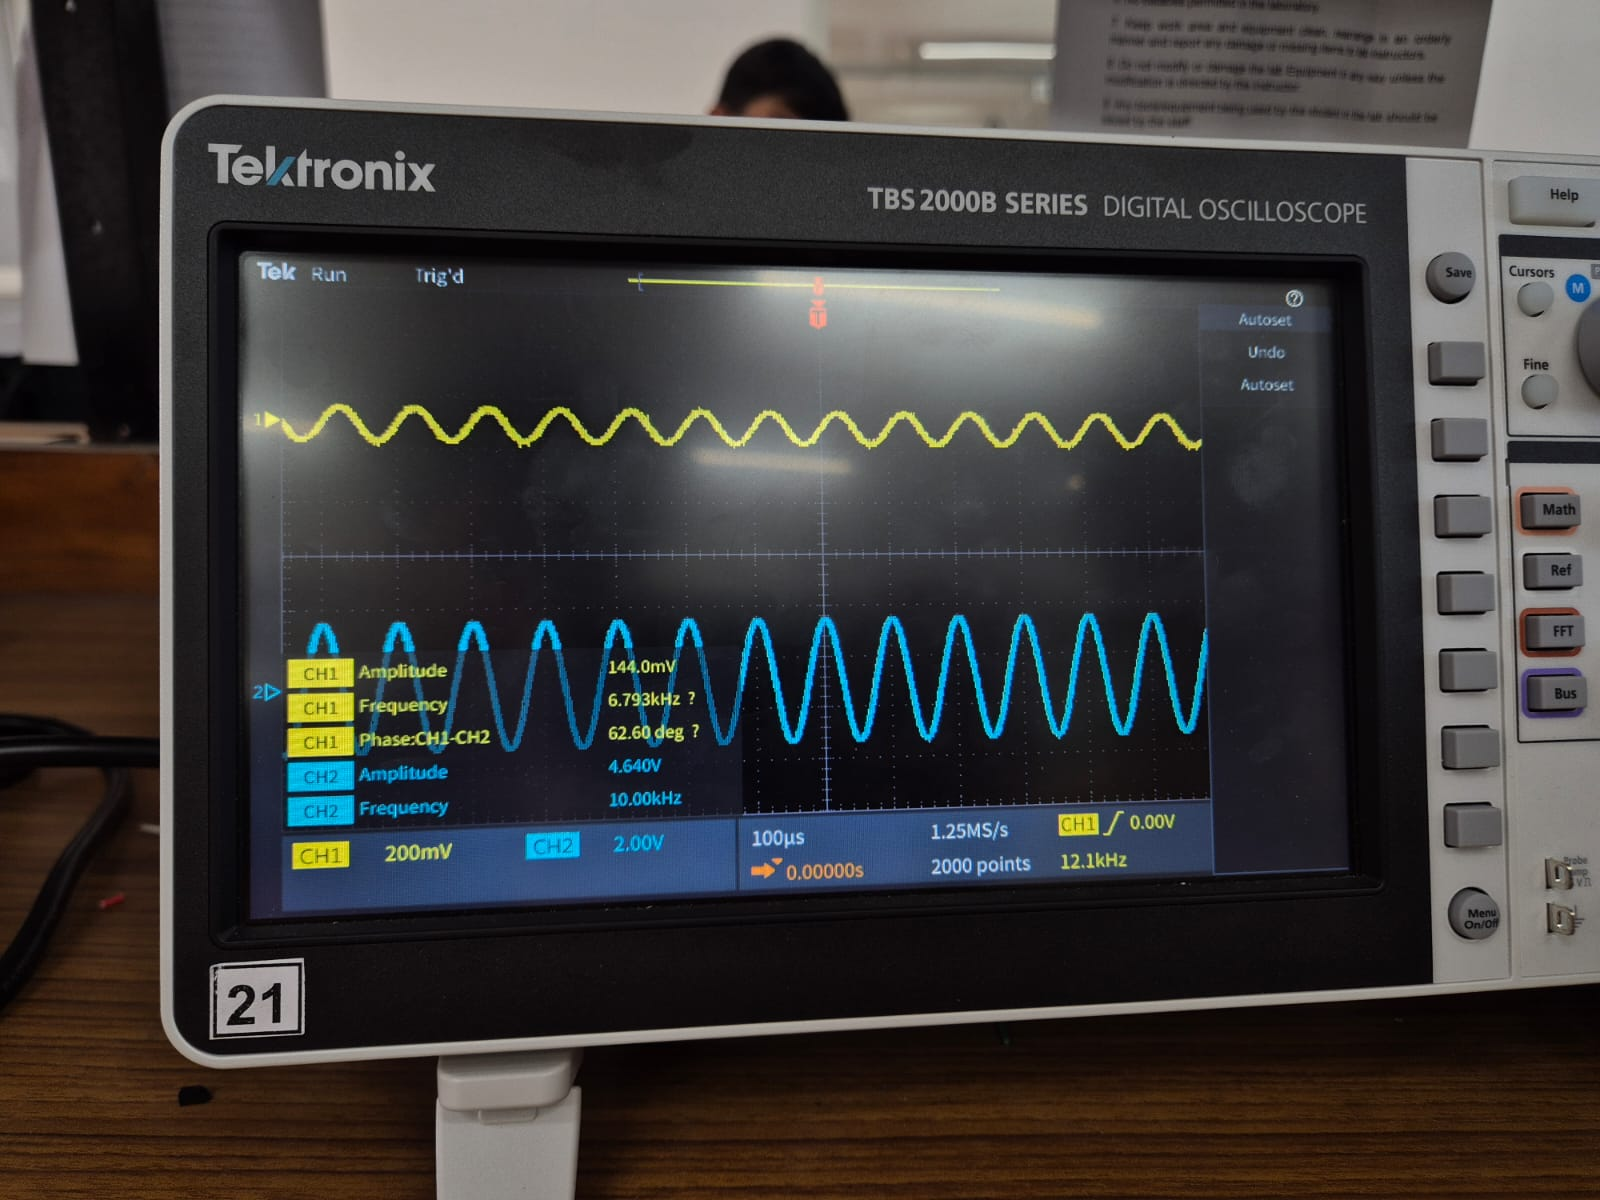
\includegraphics[width=\textwidth]{10k.jpeg}
    \caption{10kHz}
    \end{subfigure}

     \begin{subfigure}[b]{0.4\textwidth}
    \includegraphics[width=\textwidth]{100k.jpeg}
    \caption{100kHz}
    \end{subfigure}

     \begin{subfigure}[b]{0.4\textwidth}
    \includegraphics[width=\textwidth]{1M.jpeg}
    \caption{1MHz}
    \end{subfigure}
\end{figure}


\section{Conclusion}
In this experiment, the time-domain response of an RC circuit was analyzed for step, pulse, and square-wave inputs. The following observations were made:

\begin{itemize}
    \item \textbf{Step Response:} The theoretical time constant was calculated as $\tau = 0.82$ ms. The simulation yielded a perfectly matching $\tau = 0.82$ ms. The experimentally measured time constant was $\tau = 0.80$ ms, giving an error of $2.4\%$.

    \item \textbf{Pulse Response:} The circuit was tested against varying pulse widths ($200\mu s$ to $4.1$ ms). In this range, increase in pulse width led to an increase in peak voltage, as expected, due to the capacitor having more time to charge up. The experimentally obtained time constants also closely matched the theoretical value, with error averaging around $2.1\%$.

    \item \textbf{Square Wave Response:} The response of the RC circuit varied with the range of frequencies applied to the circuit. At very high frequencies, the capacitor barely charges or discharges, leading to a near 0 output, while at very low frequencies it has enough time to fully charge and thus resembles the input signal with rounded edges.
\end{itemize}

\noindent \textbf{Sources of Error:}
\begin{itemize}
    \item \textbf{Component Defects:} The actual resistance and capacitance values differed slightly from the marked $820\Omega$ and $1\mu F$ (by around $- 6\%$ and $+ 5\%$ respectively, as per multimeter).
    \item \textbf{Probe Impedance:} The internal resistance and capacitance of the oscilloscope, which has an impedance of about $50 \Omega$, was not considered here.
    \item \textbf{Measurement Accuracy:} The points on the measured waveform were measured manually and thus there is a small human error in determining $\Delta t$.
\end{itemize}
\end{document}